\documentclass{beamer}
\usetheme{Rochester}
\setbeamercovered{transparent}
\usepackage{amsfonts}
\usepackage{graphics}

\author{Yashraj Kakkad - AU1841036 \\
        Prayag Savsani - AU1841035 \\
        Harshil Mehta - AU1841010 \\
        Yashil Depani - AU1841005 \\
        \vspace{8pt}Guided by: Prof. Ashok Ranade}

\title{Music Identification through Audio Fingerprinting}

\institute{Ahmedabad University}

\date{\today}

\begin{document}

\maketitle

\begin{frame}[t] % t option for top aligned frame
\frametitle{Objective}
\begin{itemize}
    \item Extract small chunks of each song and fingerprint them.
    \item Store the chunks in an appropriate database schema. 
    \item Fingerprint a small audio sample given by user and identify the song being played.
    \item IMAGE
\end{itemize}
\end{frame}

\begin{frame}[t]
\frametitle{Sampling}
\begin{itemize}
    \item Music is typically sampled at \alert{44.1 kHz}.
    \item This is because of a theorem by \alert{Nyquist and Shannon} which requires \(f_{d} \ge 2f_{max}\).
    \item Maximum sound frequency is of course 20 kHz which leads our sampling rate to be 44.1 kHz.
\end{itemize}        
\end{frame}


\begin{frame}[t]
    \frametitle{Problems with sampling rate}
    \begin{itemize}
        \item Performing \alert{Fast Fourier Transform} on a few hundred songs takes days at such a high sampling rate.
        \item Therefore we downsample the audio by \alert{a factor of 4}. 
        \item And as a result, the maximum sound frequency in our audio sample changes to \alert{5 kHz}. 
        \item Would it cause any issues?
    \end{itemize}
\end{frame}

\begin{frame}[t]
    \frametitle{The song is not the same}   
    \begin{itemize}
        \item Turns out that the most important part of a song (to us) is below \alert{5 kHz}.
        \item Therefore, for the sake of Fast Fourier Transform, we may simply ignore the higher frequencies.
    \end{itemize}
\end{frame}
    
\begin{frame}[t]
    \frametitle{Aliasing}   
    \begin{itemize}
        \item We need to filter the higher frequencies in order to avoid aliasing.
        \item \alert{Aliasing}: Distortion that results when a signal reconstructed from samples is different from the original continuous signal.
        \item We achieve the same by filtering the signal before downsampling (using a low pass filter)
        \item IMAGE OF A LOW PASS FILTER       
    \end{itemize}
\end{frame}

\begin{frame}[t]
    \frametitle{Discrete Fourier Transform}
    \begin{itemize}
        \item Gives us the frequency spectrum.
        \item Formula: 
            \begin{align*}
                X(n) = \sum_{k=0}^{N-1} x[k] e^{-j(2\pi kn/N)}
            \end{align*}
        \item To obtain frequencies of each small part of the song for spectral analysis, we have to apply DFT on each small part of the song.
        \item This small part of the song can be seen as a window of N samples on which the DFT is performed.
        \item Such windows are extracted using a \alert{window function}.
    \end{itemize}
\end{frame}

\begin{frame}[t]
    \frametitle{Fast Fourier Transform}
    \begin{itemize}
        \item Discrete Fourier Transform requires \(\mathcal{O}(N^2)\) computations where N is the number of samples.
        \item Today's Fast Fourier Transform implementations are \(\mathcal{O}(NlogN)\), which is a huge improvement.
    \end{itemize}
\end{frame}

\begin{frame}
    \frametitle{Spectrogram}
    \begin{itemize}
        \item A three dimensional graph where:
        \begin{itemize}
            \item X-axis indicates time
            \item Y-axis indicates frequency
            \item Color indicates amplitude of a frequency at a certain time
        \end{itemize}
        \item \begin{figure}
                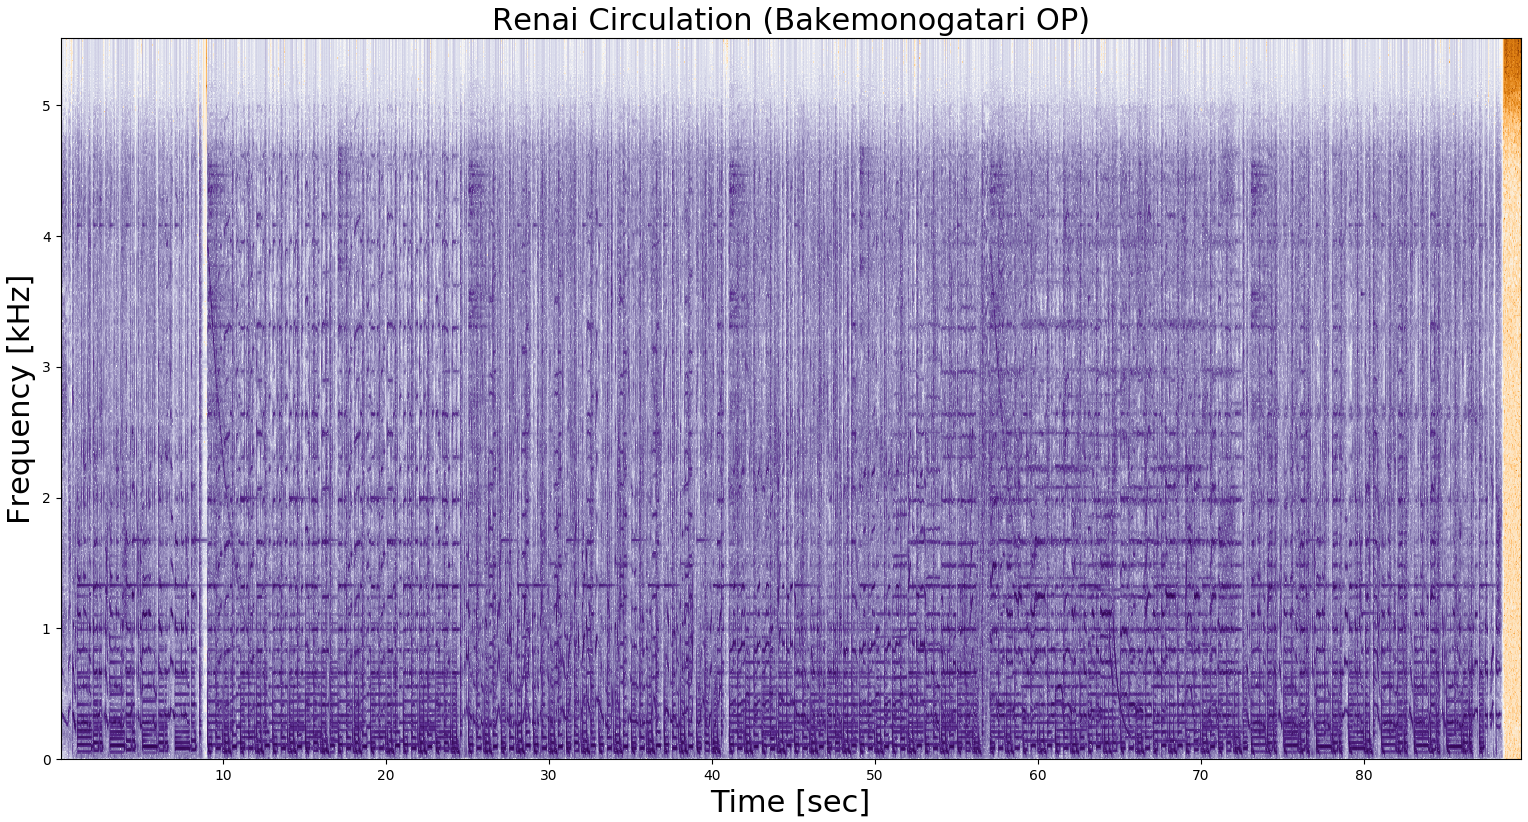
\includegraphics{Spectrogram_Specimens/ActualSong.png}
              \end{figure}
    \end{itemize}
\end{frame}

\begin{frame}
    \frametitle{Spectogram Filtering/Fingerprinting}
    \begin{itemize}
        \item We only have to keep the loudest notes
        \item Simple solution:
        \begin{itemize}
            \item For 512 bins of frequencies, we create six logarithmic bands to segregate the bins.
            \begin{itemize}
                \item very low sound band (0-10)
                \item low sound band (10-20)
                \item low-mid sound band (20-40)
                \item mid sound band (40-80)
                \item mid-high sound band (80-160)
                \item high sound band (160-511)
            \end{itemize}
            \item Keep the strongest bin of frequencies in each band.
            \item Do the same procedure to the recorded data from the user.
            % \item Then, we compute the average of strongest bins of all the windows.
            % \item You keep the bins whose magnitude is above this mean.
        \end{itemize}
    \end{itemize}    
\end{frame}

\begin{frame}
    \frametitle{Music Indexing and Matching}
    \begin{itemize}
        \item We store these frequencies as a hashed value in our database.
        \item We compare the user data with every song's data. We can compute the offset(time delay) by subtracting their positions.
        \item If we have a lot of hashes with matching offsets, we've found our song.
        % \item We compare the user data with every song's data. If we have a lot of hashes with matching values, we've found our song.
    \end{itemize}
\end{frame}

\end{document}